\chapter{A first, na{\"i}ve model}
\label{capitolo2}
\thispagestyle{empty}

\noindent A first, very simple approach to building the model for the purpose of this competition is given directly by the promoters of the challenge \cite{kernelinit}.

\bigbreak

Before seeing what the \textit{Python kernel} looks like, it's worth to dig a bit deeper on how the data is prepared for the task. In fact, taking the dataset "as it is", it's easy to notice that it has just one feature (\texttt{acoustic\textunderscore data}) that can be used to compute the regression task of predicting \texttt{time\textunderscore to\textunderscore failure} on the test set.

For this reason, data needs to be prepared: the obvious choice is to divide the training set into chunks of 150.000 rows (the size of each segment of the test set; this is not the only choice available), and for each of them compute some features representing the data; in this first basic solution we will extract the mean, standard deviation, maximum and minimum. The resulting dataset will contain an entry for each portion of the initial dataset, with one column for each computed feature (in this case 4), and another dataset with just the original \texttt{time\textunderscore to\textunderscore failure} associated with the last row of the chunk (similarly to the test segments).

\section{Basic Feature Benchmark}
\begin{lstlisting}
# This Python 3 environment comes with many helpful analytics libraries installed
# It is defined by the kaggle/python docker image: https://github.com/kaggle/docker-python
# For example, here's several helpful packages to load in 

import numpy as np # linear algebra
import pandas as pd # data processing, CSV file I/O (e.g. pd.read_csv)

# Input data files are available in the "../input/" directory.
# For example, running this (by clicking run or pressing Shift+Enter) will list the files in the input directory

import os
print(os.listdir("../input"))

# Any results you write to the current directory are saved as output.
\end{lstlisting}

\begin{lstlisting}[firstnumber=15]
import matplotlib.pyplot as plt
from tqdm import tqdm
from sklearn.preprocessing import StandardScaler
from sklearn.svm import NuSVR
from sklearn.metrics import mean_absolute_error
\end{lstlisting}

\begin{lstlisting}[firstnumber=20]
train = pd.read_csv('../input/train.csv', dtype={'acoustic_data': np.int16, 'time_to_failure': np.float64})
\end{lstlisting}

After these preliminary operations of including the necessary libraries and loading the dataset, we are able to get into the data preparation as previously described. In the following snippet, \texttt{X\_train} is the dataset containing the segments' 4 computed features, while \texttt{Y\_train} contains the associated \texttt{time\textunderscore to\textunderscore failure}.

\begin{lstlisting}[firstnumber=21]
# Create a training file with simple derived features

rows = 150_000
segments = int(np.floor(train.shape[0] / rows))

X_train = pd.DataFrame(index=range(segments), dtype=np.float64,
                       columns=['ave', 'std', 'max', 'min'])
y_train = pd.DataFrame(index=range(segments), dtype=np.float64,
                       columns=['time_to_failure'])

for segment in tqdm(range(segments)):
    seg = train.iloc[segment*rows:segment*rows+rows]
    x = seg['acoustic_data'].values
    y = seg['time_to_failure'].values[-1]
    
    y_train.loc[segment, 'time_to_failure'] = y
    
    X_train.loc[segment, 'ave'] = x.mean()
    X_train.loc[segment, 'std'] = x.std()
    X_train.loc[segment, 'max'] = x.max()
    X_train.loc[segment, 'min'] = x.min()
\end{lstlisting}

The kernel's authors' choice for modeling the solution is to use \textit{Support Vector Regression}. The \texttt{scikit-learn} Python library implementation of SVR recommends explicitly that the data is scaled, since Support Vector Machine algorithms are not scale invariant.

\begin{lstlisting}[firstnumber=42]
scaler = StandardScaler()
scaler.fit(X_train)
X_train_scaled = scaler.transform(X_train)
\end{lstlisting}

\begin{lstlisting}[firstnumber=45]
svm = NuSVR()
svm.fit(X_train_scaled, y_train.values.flatten())
y_pred = svm.predict(X_train_scaled)
\end{lstlisting}

The results predicted are then compared with the actual training data, by computing the \textit{Mean Absolute Error}, and finally the test data is prepared and fed to the model and results are printed to the \texttt{submission.csv} file. As expected, this simple model has a score of 2,314 on the training set (the score on the test set can only be computed by the competition's promoters), which denotes a really bad performance.

\begin{lstlisting}[firstnumber=48]
score = mean_absolute_error(y_train.values.flatten(), y_pred)
print(f'Score: {score:0.3f}')
\end{lstlisting}

\begin{lstlisting}[firstnumber=50]
submission = pd.read_csv('../input/sample_submission.csv', index_col='seg_id')
X_test = pd.DataFrame(columns=X_train.columns, dtype=np.float64, index=submission.index)
\end{lstlisting}

\begin{lstlisting}[firstnumber=52]
for seg_id in X_test.index:
    seg = pd.read_csv('../input/test/' + seg_id + '.csv')
    
    x = seg['acoustic_data'].values
    
    X_test.loc[seg_id, 'ave'] = x.mean()
    X_test.loc[seg_id, 'std'] = x.std()
    X_test.loc[seg_id, 'max'] = x.max()
    X_test.loc[seg_id, 'min'] = x.min()
\end{lstlisting}

\begin{lstlisting}[firstnumber=61]
X_test_scaled = scaler.transform(X_test)
submission['time_to_failure'] = svm.predict(X_test_scaled)
submission.to_csv('submission.csv')
\end{lstlisting}

\begin{figure} [h]
	\centering
	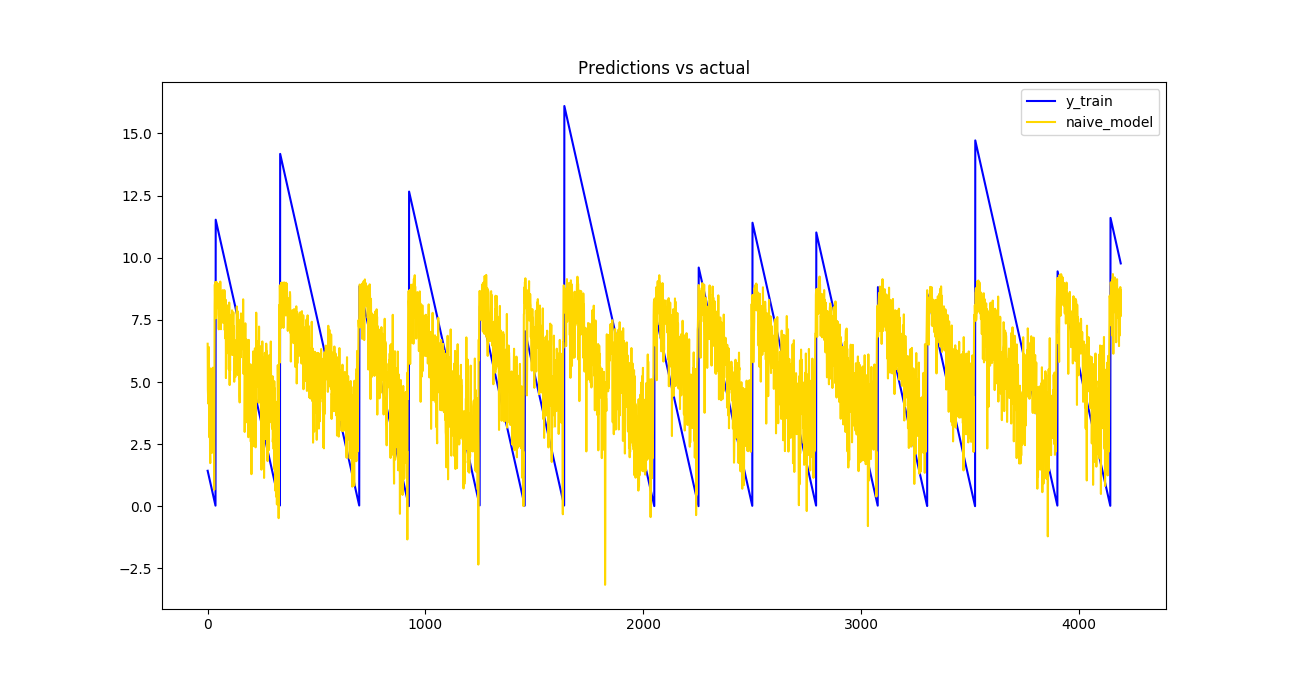
\includegraphics[width=1\linewidth]{pictures/naive.png}
	\caption{Na{\"i}ve model, \texttt{time\textunderscore to\textunderscore failure} predictions vs real values.}
	\label{fig:LR}
\end{figure}